\documentclass[a4paper,11pt]{memoir}                                        

\usepackage[utf8]{inputenc}
\usepackage[danish]{babel}
\usepackage[T1]{fontenc}
\usepackage[left=0.8in, right=0.8in, top=1.0in, bottom=1.0in]{geometry} 
\usepackage{amsmath,amssymb}																						

% SIUnitX  http://ctan.org/pkg/siunitx
\usepackage{siunitx,booktabs}		
\sisetup{per=slash}																						
\sisetup{per-mode = reciprocal}
\sisetup{inter-unit-product = \ensuremath{{}\cdot{}}}
\sisetup{output-decimal-marker = {,} }
\DeclareSIUnit{\kroner}{kr.}

\usepackage{graphicx}
\newsubfloat{figure}% Allow subfloats in figure environment
\usepackage{dcolumn,booktabs}
\usepackage{url}
\usepackage{wrapfig}

% Redigere billed-/tabelteksterne.
\usepackage{caption}
\usepackage{subcaption}
\captionsetup{font=small,
labelfont={it,bf},textfont=sf,
format=hang}

% Packages for color handling
\usepackage[usenames,dvipsnames,svgnames,table]{xcolor}

\usepackage{threeparttable}

\usepackage[hidelinks]{hyperref}  
\hypersetup{bookmarks=false}
\hypersetup{pdftitle={Inverteret Pendul}} 
\hypersetup{pdfsubject={3. Semester Projekt, E-EEP (Elektromagnetisme, Elektronik og Projekt) og E-RMK (Regulering, Matematik og Kredsløbsteknik) E16, Grp. [4]}}
\hypersetup{pdfauthor={J\"{o}rn Jacobi, Simon Møller, Søren Frank, Nikolaj Kyed, Kenneth Petersen, Benjamin Lund}}


% TODONotes http://ctan.org/pkg/todonotes
\usepackage{todonotes}
\usepackage{placeins}

% For includering af .pdf
\usepackage{pdfpages}

% Bibliografi
\usepackage{babelbib}
\bibliographystyle{abbrv}

% Noget forsideopsætning
\usepackage{soul} % lege lege
\sodef\an{}{0.2em}{.9em plus.6em}{1em plus.1em minus.1em}
\newcommand\stext[1]{\an{\scshape#1}}

% New commands 
\newcommand{\g}{9,82 \si{\meter\per\second\squared}}
\newcommand{\dcite}[1]{\quotedblbase{#1}\textquotedblright}
\newcommand{\husk}[2]{\todo[inline,color=green!40]{#1: #2}}
\DeclareMathOperator{\lapl}{\mathcal{L}}
% Remove paragraph indentation for document
\setlength{\parindent}{0pt}
\newcommand\hcancel[2][black]{\setbox0=\hbox{$#2$}%
	\rlap{\raisebox{.45\ht0}{\textcolor{#1}{\rule{\wd0}{1pt}}}}#2} 

% Listings package
\usepackage{listings}


%Fede overskrifter
\usepackage{kpfonts}
\usepackage{calc}
\setSingleSpace{1.0}
\SingleSpacing
\definecolor{chaptercolor}{gray}{0.8}
% helper macros
\newcommand\numlifter[1]{\raisebox{-2cm}[0pt][0pt]{\smash{#1}}}
\newcommand\numindent{\kern37pt}
\newlength\chaptertitleboxheight
\makechapterstyle{hansen}{
  \renewcommand\printchaptername{\raggedleft}
  \renewcommand\printchapternum{%
    \begingroup%
    \leavevmode%
    \chapnumfont%
    \strut%
    \numlifter{\thechapter}%
    \numindent%
\endgroup%
}
  \renewcommand*{\printchapternonum}{%
    \vphantom{\begingroup%
      \leavevmode%
      \chapnumfont%
      \numlifter{\vphantom{9}}%
      \numindent%
      \endgroup}
    \afterchapternum}
  \setlength\midchapskip{0pt}
  \setlength\beforechapskip{0.5\baselineskip}
  \setlength{\afterchapskip}{1\baselineskip}
  \renewcommand\chapnumfont{%
    \fontsize{3cm}{0cm}%
    \bfseries%
    \sffamily%
    \color{chaptercolor}%
  }
  \renewcommand\chaptitlefont{%
    \normalfont%
    \huge%
    \bfseries%
    \raggedleft%
  }%
  \settototalheight\chaptertitleboxheight{%
    \parbox{\textwidth}{\chaptitlefont \strut bg\\bg\strut}}
  \renewcommand\printchaptertitle[1]{%
    \parbox[t][\chaptertitleboxheight][t]{\textwidth}{%
      %\microtypesetup{protrusion=false}% add this if you use microtype
      \chaptitlefont\strut ##1\strut}%
}}
\chapterstyle{hansen}
\aliaspagestyle{chapter}{empty} % just to save some space





\begin{document}
\begin{titlingpage}
\thispagestyle{empty}
\centering
{ \setlength{\baselineskip}{24pt}
{\Huge \stext{Inverteret Pendul} \par
%\textit{\&}\par
%\stext{Analogier}
}\par
\stext{E-EEP og E-RMK E16}
\par\vspace*{4\onelineskip}
\par

\includegraphics[width=10cm]{billeder/SDU_segl1.png}
\par\vspace*{4\onelineskip}
\stext{3. Semester Projekt}\par

\large\stext{J\"{o}rn Jacobi -- 230674}\par
\large\stext{Simon M\o ller -- 230893}\par
\large\stext{S\o ren Frank -- ddmmyy}\par
\large\stext{Nikolaj Kyed -- ddmmyy}\par
\large\stext{Kenneth Petersen -- ddmmyy}\par
\large\stext{Benjamin Lund -- ddmmyy}\par

\vfill
\vspace*{2\onelineskip}
\stext{Vejleder: Kurt B. Jessen}\par
\stext{1. september - 19. december 2016}\hfill
%\stext{24. maj 2013}\hfill
\par\vspace*{2\onelineskip}
\small
\stext{M\ae rsk Mc-Kinney M\o ller Instituttet}\par
\stext{Syddansk Universitet}
\enlargethispage{2\onelineskip}
}
\end{titlingpage}
\newpage

\renewcommand{\abstractnamefont}{\normalfont\bfseries}
\renewcommand{\abstracttextfont}{\normalfont}

\begin{abstract}
Resume her... 	
\end{abstract}

\thispagestyle{empty}

%---------- Indholdsfortegnelse  ---
\newpage
\thispagestyle{empty}
\null
\vfill
\begin{center}
\emph{Tak til, hvis nogen ...}
\end{center}
\newpage
\thispagestyle{empty}
\null

\section*{Underskrifter}
\vspace{3ex} \hfill Underskrevet d. xx/12-2016\\

\newlength{\streg} \setlength{\streg}{0.49\linewidth}
\vspace*{\fill} \rule{\streg}{1pt} \hfill \rule{\streg}{1pt}\\
\begin{minipage}[b]{\streg}
 \centering
 \rule{0pt}{4ex}
 J\"{o}rn Jacobi \\
 {\footnotesize (230674) (jojac11@student.sdu.dk)}
\end{minipage}
\hfill
\begin{minipage}[b]{\streg}
 \centering
 Simon Møller \\
 {\footnotesize (ddmmyy) (navn@student.sdu.dk)}
\end{minipage}

\vspace*{\fill} \rule{\streg}{1pt} \hfill \rule{\streg}{1pt}\\
\begin{minipage}[b]{\streg}
 \centering
 \rule{0pt}{4ex}
 Søren Frank \\
 {\footnotesize (300595) (sofra15@student.sdu.dk)}
\end{minipage}
\hfill
\begin{minipage}[b]{\streg}
 \centering
 Nikolaj Kyed \\
 {\footnotesize (ddmmyy) (navn@student.sdu.dk)}
\end{minipage}

\vspace*{\fill} \rule{\streg}{1pt} \hfill \rule{\streg}{1pt}\\
\begin{minipage}[b]{\streg}
	\centering
	\rule{0pt}{4ex}
	Kenneth Petersen \\
	{\footnotesize (ddmmyy) (navn@student.sdu.dk)}
\end{minipage}
\hfill
\begin{minipage}[b]{\streg}
	\centering
	Benjamin Lund \\
	{\footnotesize (ddmmyy) (navn@student.sdu.dk)}
\end{minipage}	
\newpage
\thispagestyle{empty}
\null
\vfill
\newpage
\tableofcontents*												
\newpage

\DoubleSpacing
%---------- Kalibrerings side --------
%Lorem ipsum dolor sit amet, pri ipsum partiendo interpretaris ea. Eum meliore persecuti no, at fugit quando mei. Nibh aliquid cum ei. Ne utinam libris nec, ex aliquip antiopam pri. Nam assum affert ancillae an, eos ea hinc mundi, dolor eleifend volutpat no usu. Ut nam esse essent ponderum. Ut eam quidam partiendo deterruisset, te pri consequuntur concludaturque. In oportere abhorreant vis, in usu ludus graeco volutpat, vel iudico dicunt prodesset ea. Mei natum noster eu, mei no ornatus ocurreret.
Pri unum maiestatis in, agam audiam perfecto ne mel. Ut per invenire petentium adolescens. An mei propriae phaedrum postulant. Vim amet electram ei. Ea wisi dolorem qui, mea propriae persecuti ad, option nusquam nominati ut mei. Nam te animal inermis, verear neglegentur ius id. His quem prompta inermis id, eruditi invidunt vix id. Eu sea tota vidisse deseruisse, aliquid nostrum voluptua ea vel. Facete audiam abhorreant an eum. Vim magna appellantur ne, vidit nulla sed ut. Mei nostrum vituperata consectetuer no. Noluisse placerat salutandi qui eu. Cum eu illud clita. Est vivendum convenire ex, sit primis iriure neglegentur an, ex sed modus tincidunt. Evertitur pertinacia constituam eu mea. Oblique alienum ocurreret ius ad. In eos aeterno iuvaret liberavisse, accusata euripidis an per. Nibh detracto placerat sea ut. Pri an minim aperiam omnesque, ancillae appareat reformidans ius in. Cibo aeterno erroribus ut eam, vim recteque scribentur liberavisse eu, choro soluta dolorem vis ea. Ad vel nullam graece legendos, sit melius menandri expetenda at. Sea inermis dolores ad, ut has noster argumentum. Qui movet zril an, in nam nobis quando. Usu ne saperet nostrum, per te nominati accusamus sententiae, est cu debet virtute accusata. Nihil fastidii his cu, pri aeterno persius vivendo id. Per te wisi temporibus, ullum iudicabit mea te, duis recusabo ea vel. Vim quodsi accumsan ut, te pro explicari iracundia. Vim id molestiae posidonium, clita everti facilisis ius te. Cu adhuc convenire comprehensam vis, decore facilis torquatos qui ne, at qui duis legendos sarium.
Zril commodo theophrastus cu cum. Eu reformidans conclusionemque sit, vix eu cibo everti similique, ex duo munere omnium principes. An vel sapientem moderatius, malis lobortis partiendo vel ne. Ea quod graeci expetenda usu.
Denne tekst er skrevet med Century Schoolbook fontstørrelse 11, med en afstand på 8pkt. efter afsnit og linjeafstand på 1.5.
%\newpage

%---------- Indledning -------------
\chapter{Indledning}

\section{Forord}\label{sec:forord}
Udarbejdningen af dette projekt er blevet udført af studerende i Gruppe 4 på 3. semester ved Syddansk Universitet, Teknisk Fakultet fra uddannelserne elektronik og datateknik samt elektrisk energiteknologi, Efterår 2016.
Projektet er en sammenfatning af de opnåede fagligheder fra semesterets undervisning: elektronik, elektromagnetisme, regulering, kredsløbsteknik og matematik.

Projektet går ud på at balancere en stang i et én dimensionelt rum ved hjælp af en vogn. Under projektforløbet har gruppen valgt, at uddeligere arbejdesopgaverne. Simon og Søren tog sig af det elektromagnetiske, hvor de fik designet spolerne og spoleholderne. Kenneth og Nikolaj fik lavet kredsløbene der gjorde det muligt, at få et brugbart signal til motorstyringen. Jörn analyserede det fysiske system; pendulets bevægelse i forhold til bilen, derudover motorstyringen og dimensioneringen af regulatoren.

Under hele projektforløbet har gruppen fulgt med i den enkeltes arbejdsopgaver, dels for at hjælpe hinanden og for at få en bedre samlet forståelse af projektet, og ikke mindst for at holde overblik i forhold til tidsplanen. 
\\ \\
Rapporten er bestående af samlet \pageref{LastPage} sider, heraf  9 tomme sider grundet layoutmæssige valg. 
% !TeX root = ../rapport.tex
\chapter{Indledning}

\section{Problemformulering}
At designe og fremstille et éndimensionelt vognmonteret omvendt pendul, der ved hjælp af regulering skal kunne fastholde en forudbestemt vinkel af pendulet, samt at kunne kompensere for udefrakommende påvirkninger. 

\subsection{Formål}
Formålet med projektet er, at forene de opnåede fagligheder fra undervisningen på 3. semester for elektronik og datateknik og for stærkstrøm. Alle fag fra undervisningen indgår i projektet, og er henholdsvis elektronik, elektromagnetisme, regulering, kredsløbsteknik og matematik.

\subsection{Krav til rapporten stillet i projektoplæg}
Måling og generering af elektromagnetiske felter kombineret med analog signalbehandling.
\husk{JJ}{Husk at opdatere projektoplægs krav inkl. ref. til oplæg}
\begin{itemize}
\item E-EEP (Elektromagnetisme, Elektronik og Projekt).
\item E-RMK (Regulering, Matematik og Kredsløbsteknik).
\end{itemize}

\subsection{Selvvalgte krav til produktet} \label{afs:kravspecifikation}
\begin{itemize}
\item Systemet skal kunne opretholde en maksimal svingvinkel af pendulet på 20 grader.
\item (Masser af systemet)
\item Systemet skal kunne drives af et/to batteri(er)
\item Sensoren skal være induktiv
\end{itemize}

\subsection{Problemstilling}
Følgende problemstillinger ønskes besvaret:
\begin{itemize}
\item Første
\item Anden
\end{itemize}

\subsection{Projektafgrænsning}
Følgende medtages ikke i rapporten og afgrænser projektarbejdet:
\begin{itemize}
\item Systemet skal kun virke i én retning (dimension)
\item Der ses bort fra fysisk beskrivelse af elektromotoren.
\item Der ses bort fra beskrivelsen af motorstyringen.
\item Vogn samt tilhørende motor, hjul og gearing overtages fra tidligere projekt.
\end{itemize}

\section{Løsningsmodel}
Blokdiagrammet her ?
\husk{JJ}{Del diagram af system og signalvej ?}

\section{Læsevejledning}
Rapportens læsevejledning...\\
Naturlig indførelse i emnet

\section{Arbejdsmetode}
Noter til arbejdsmetoden.
\begin{itemize}
	\item Iterativ planlægning
	\item ugentlige status møder hvor der opsummeres
	\item fleksibel opgave styring, for maksimal udnyttelse af ressourcer 
	\item To-Do lister
\end{itemize}

\section{Blokdiagram}
\begin{figure}[h!]
	\centering
	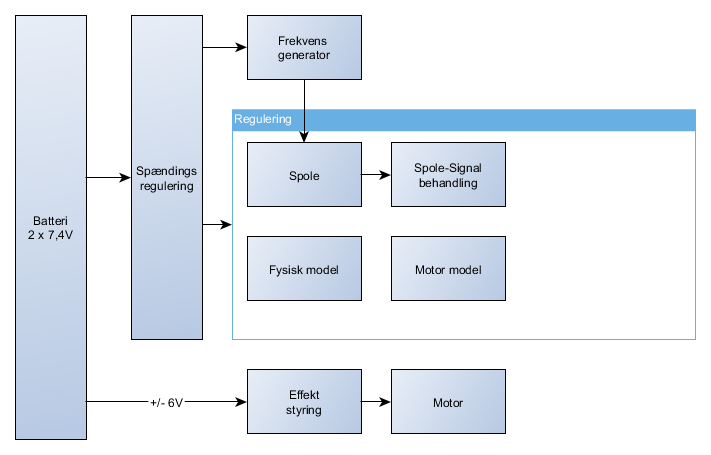
\includegraphics[width=.9\textwidth]{diagram/blokdiagram1.png}
	\caption{System blokdiagram.}
	\label{fig:blockdiagram1}
\end{figure}
\FloatBlock




							

\listoftodos
%\newpage
\section{How To do stuff in LaTeX}

\subsection*{Figur, enkelt}
%-----------------------------------------------------------------------------
\begin{figure}[h!]
	\centering
		\includegraphics[width=.5\textwidth]{billeder/sample.png}
	\caption{Her skrives en god caption til figuren.}
	\label{fig:sample_fig_ref_her}
\end{figure}
\FloatBlock
%-----------------------------------------------------------------------------

\subsection*{Figur, dobbelt}
%-----------------------------------------------------------------------------
\begin{figure}
	\centering
	\subbottom[]{%
  		\includegraphics[width=.39\textwidth]{billeder/sample.png}
	  	\label{fig:sample_fig_ref_her_a}}
	\subbottom[]{%
		\includegraphics[width=.39\textwidth]{billeder/sample.png}
		\label{fig:sample_fig_ref_her_b}}
  	\caption{Her skrives en god caption til figuren.}
	\label{fig:sample_fig_ref_her_samlet}
\end{figure}
\FloatBlock
%-----------------------------------------------------------------------------

\subsection*{Kommentar}
%-----------------------------------------------------------------------------
\husk{Initialer}{Kommentaren skrives her}
%-----------------------------------------------------------------------------

\subsection*{Math Simple}
%-----------------------------------------------------------------------------
\begin{align}
D = \frac{1}{\Delta F}
\end{align}
%-----------------------------------------------------------------------------

\subsection*{Math uden nummer og align}
%-----------------------------------------------------------------------------
\begin{align}
D &= \frac{1}{\Delta F} \Rightarrow \nonumber \\
\Omega &= \mathrm{Noget helt andet}
\end{align}
%-----------------------------------------------------------------------------
\subsection*{Tabeller med caption}
\begin{table}
\centering
    \caption{Konstanter som bruges i overstående formler.}
\label{tab:konst1}
    \begin{tabular}{ | l | l |}
    \hline
    A & 18 [V] \\ \hline
    f & 50 [Hz]  \\ \hline
    T & 20 [s]  \\ \hline
    $\omega$ & 30 \\ \hline
    k & 100 \\ \hline
    \end{tabular}
    \end{table}

\newpage

%---------- Chapter ----------------
\chapter{Fysisk model og dens overførelses funktion}\label{kap:chap_fysik_reg}

\emph{Introduktion til emnet i kapitlet skrives her}


%---------- Parts ----------------
\section{Fritlegemediagram og analyse af pendul}\label{sec:sec_fritlegemediagram}

\begin{wrapfigure}{r}{0.4\textwidth}
	\centering
	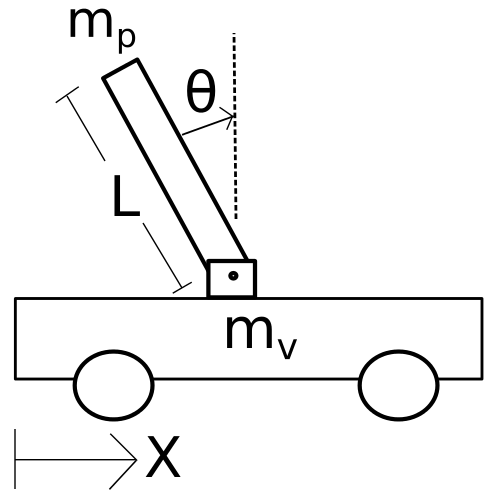
\includegraphics[width=.3\textwidth]{billeder/pendul_vogn.png}
	\caption{Simpel model af pendul og vogn.}
	\label{fig:pendul_vogn}
\end{wrapfigure}
\FloatBlock

Det inverterede pendul er monteret på en vogn med hjul, som vist i figur \ref{fig:pendul_vogn}.
Således er det muligt at flytte vognen samtidig med at der er fri bevægelse af pendulet rundt om pendulets rotations punkt, der er fastgjort på vognen.
Der er således kun tale om én-dimensional bevægelse af vognen.

Det vælges at analysere pendulet og vognen hver for sig.
Pendulet anses som en masseløs stang hvor massen er fastgjort for enden af stangen. 
Således angiver $T$ den trækkraft der er mellem vogn og pendul.
\begin{figure}
	\centering
	\subbottom[]{%
		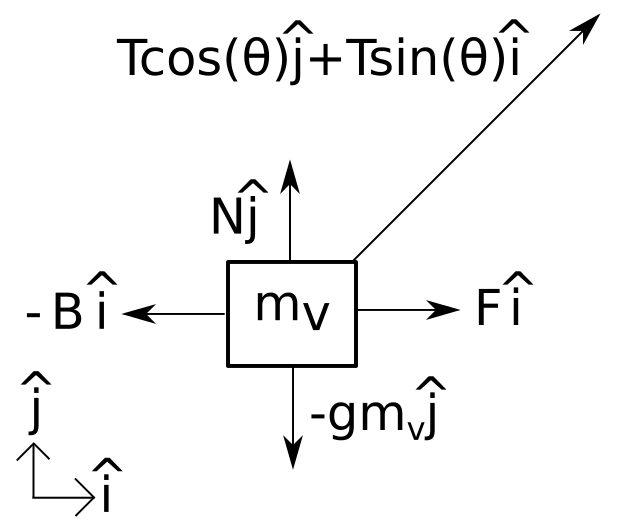
\includegraphics[width=.39\textwidth]{billeder/fridiagram_vogn.png}
		\label{fig:fridiagram_vogn}}
	\subbottom[]{%
		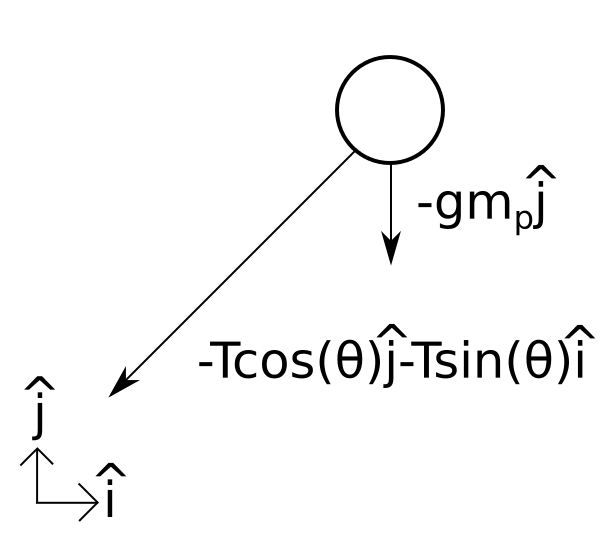
\includegraphics[width=.39\textwidth]{billeder/fridiagram_pendul.png}
		\label{fig:fridiagram_pendul}}
	\caption[Frit-legeme digrammer af vogn og pendul]{Frit-legeme diagrammer af henholdsvis vogn (a) og pendul (b).}
	\label{fig:fridiagrammer}
\end{figure}

Opsummering af kræfter på vognen som ses i frit-legeme diagrammet i figur \ref{fig:fridiagram_vogn}. 
\begin{alignat}{3}
&\hat{i} : \quad && F_c + T sin{\theta} && = m_v \ddot{x} \label{eq:vogn_x}\\
&\hat{j} : \quad && -g m_v + N && = 0 
\end{alignat}

Opsummering af kræfter på pendulet som ses i frit-legeme diagrammet i figur \ref{fig:fridiagram_pendul}.
\begin{alignat}{3}
&\hat{i} : \quad &&-T sin{\theta} &&= m_p a_{px}\label{eq:apx}\\
&\hat{j} : \quad &&-T cos{\theta} - m_p g &&= m_p a_{py}\label{eq:apy} 
\end{alignat}

\begin{wrapfigure}{r}{0.4\textwidth}
	\centering
	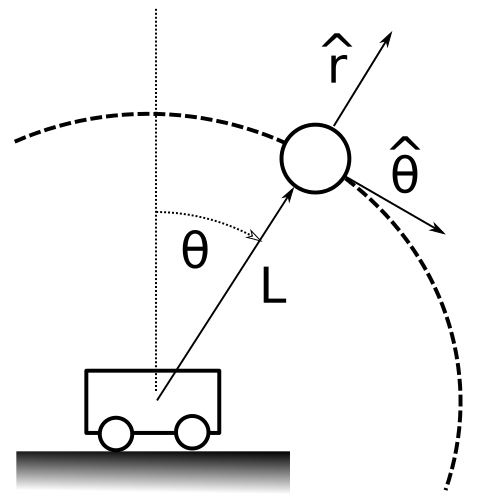
\includegraphics[width=.3\textwidth]{billeder/pendul_vogn_polaer.png}
	\caption{Retnings angivelse for polær koordinater på pendul.}
	\label{fig:pendul_vogn_polaer}
\end{wrapfigure}

Den relative acceleration af pendulet udledes i polær koordinater med retnings reference som angivet i figur \ref{fig:pendul_vogn_polaer}. 
\begin{align}
\vec{a}_p &= \vec{a}_v + \vec{a}_{p/v} \\
&= \ddot{x} \hat{i} + \left( L\ddot{\theta}\hat{\theta} - L\dot{\theta}^2\hat{r} \right)
\end{align}

Accelerationsvektoren $\vec{a}_p$, for pendulet omskrives nu fra polær-koordinator til kartesiske koordinator  
\begin{align}
\vec{a}_p &=  \ddot{x} \hat{i} 
				+ L\ddot{\theta} \left( \cos{\theta}\hat{i} - \sin{\theta}\hat{j} \right) 
				- L\dot{\theta}^2 \left( \sin{\theta}\hat{i} + \cos{\theta}\hat{j} \right) \label{eq:ap}
\end{align} 

Accelerationen for pendulet, $\vec{a}_{px}$ og $\vec{a}_{py}$, i ligning \ref{eq:apx} og \ref{eq:apy} kan nu erstattes, med den relative acceleration fundet i ligning \ref{eq:ap}
\begin{align}
-T\sin{\theta} &= m_p \left( \ddot{x} + L\ddot{\theta}\cos{\theta} - L\dot{\theta}^2\sin{\theta} \right)  \label{eq:pendul_x2}\\
-T\cos{\theta} - m_p g &=  -m_p \left( L\ddot{\theta}\sin{\theta} + L\dot{\theta}^2\cos{\theta}  \right) \label{eq:pendul_y2}
\end{align} 

Trækkræfter $T$ fjernes fra pendul ligningerne \ref{eq:pendul_x2} og \ref{eq:pendul_y2} ved gensidig at gange med $-\cos{\theta}$ og $\sin{\theta}$. 
\begin{align}
T\sin{\theta}\cos{\theta} &=   -m_p \cos{\theta} \left( \ddot{x} + L\ddot{\theta}\cos{\theta} - L\dot{\theta}^2\sin{\theta} \right) \label{eq:pendul_x3} \\
-T\cos{\theta}\sin{\theta} - m_p g &=  -m_p \sin{\theta} \left( L\ddot{\theta}\sin{\theta} + L\dot{\theta}^2\cos{\theta}\right) \label{eq:pendul_y3}
\end{align}

Ligning \ref{eq:pendul_x3} og \ref{eq:pendul_y3} adderes
\begin{align}
-m_p g \sin{\theta}    &= - m_p \ddot{x}\cos{\theta}
						- m_p L\ddot{\theta}\cos^2\theta\
						\hcancel[red]{+ m_p L \dot{\theta}^2\cos{\theta}\sin{\theta}}\\
					   &\quad - m_p L\ddot{\theta}\sin^2\theta\
					    \hcancel[red]{- m_p L \dot{\theta}^2\cos{\theta}\sin{\theta}} \\
					   &=- m_p \cos{\theta}\ddot{x} - m_p L \ddot{\theta} \left(\sin^2 \theta \cos^2 \theta \right) \\
					   &=- m_p \cos{\theta}\ddot{x} - m_p L \ddot{\theta} \label{eq:pendul_mellem}
\end{align}

I ligning \ref{eq:vogn_x} fjernes $T$ ved at substituere med ligning \ref{eq:pendul_x2}
\begin{align}
F_c - m_p \ddot{x} - m_p L\ddot{\theta}\cos{\theta} + m_p L\dot{\theta}^2\sin{\theta} &= m_v \ddot{x} \Leftrightarrow \\
F_c - m_p L\ddot{\theta}\cos{\theta} + m_p L\dot{\theta}^2\sin{\theta} &= (m_v + m_p)  \ddot{x} \label{eq:vogn_mellem}
\end{align}

Ligningerne af det fysiske system for pendul og vogn fremstår i nu i \ref{eq:pendul_mellem} og \ref{eq:vogn_mellem}. Disse to ligninger er ikke lineære. En forudsætning for at kunne gennemføre en linearisering er at antage, at udefrakommende påvirkninger til systemet er så små, at små forstyrrelser kun give anledning til små ændringer af vinkelen $\theta$ og en approksimmering kan antages som
\begin{align}
\sin{\theta} \approxeq \theta \quad og \cos{\theta} \approxeq 1
\end{align} 

Ligeledes kan udtrykket $\dot{\theta}^2$ reduceres til
\begin{align}
\dot{\theta}^2 = \left( \dfrac{d}{dt}\theta \right)^2 =  \left( \dfrac{d}{dt}\sin{\theta} \right)^2 = \left(\cos{\theta}\right)^2 \approxeq (1)^2 = 1
\end{align}

Det ønskes at få et udtryk der forbinder position $x$ med vinklen $\theta$ for pendulet, så ligning \ref{eq:pendul_mellem} forkortes. Pendulets masse $m_p$ forkortes også bort. 
\begin{align}
-m_pg\theta &= -m_p\ddot{x}-m_p L \ddot{\theta} \Leftrightarrow\\
\ddot{x} &= g \theta -L \ddot{\theta} \label{eq:pendul_lin}
\end{align}

Nu tages \ref{eq:pendul_lin} og indsættes i ligning \ref{eq:vogn_mellem}
\begin{align}
F_c - m_p L\ddot{\theta} + m_p L\theta &= (m_v + m_p)(g \theta -L \ddot{\theta})  \\
F_c  - m_p L\ddot{\theta} + m_p L\theta &= m_v g \theta +  m_p g \theta - m_v L \ddot{\theta} - m_p L \ddot{\theta}
\end{align}

I ovenstående udtryk, erstattes $F_c = ma_v$ for og reduceres
\begin{align}
m a_v - \hcancel[red]{ m_p L\ddot{\theta}} + m_p L\theta &= (m_v + m_p) g \theta - m_v L \ddot{\theta} - \hcancel[red]{ m_p L\ddot{\theta}} \Leftrightarrow \\
m_v L \ddot{\theta} - m g \theta &= - m_p L\theta -m a_v \label{eq:system_final}
\end{align} 

Ligning \ref{eq:system_final} er således den endelige beskrivelse af pendul og vogn hvori systemets overførelses funktion kan findes.
På højre side ses de eksterne forstyrrelser. 
$m_pL\theta $ er påvirkningen af en lille ændring af pendulet, og $m a_v$ er en ændring i vognens acceleration.
\section{Overførelsesfunktion af pendulet}\label{sec:sec_penduloverforelse}
Ved at Laplace-transformere ligningen \ref{eq:system_final}, findes $\theta(s)$
\begin{align}
 m_vLs^2\theta(s) - mg = -m_pL\theta(s) -mA_v(s) \\
 \theta(s)\left(m_vLs^2 - mg \right) = -m_pL\theta(s) -mA_v(s) \\
 \theta(s) = \frac{1}{m_vLs^2 - mg }\left[-m_pL\theta(s) -mA_v(s)\right] \label{eq:pendul_final}
\end{align} 
 
Ved at opstille overførelsesfunktionen i ligning \ref{eq:pendul_final} som model i figur \ref{fig:pendul_trans1}, fremgår de ind- og udgående variabler tydeligt. 

\begin{figure}[h!]
	\centering
	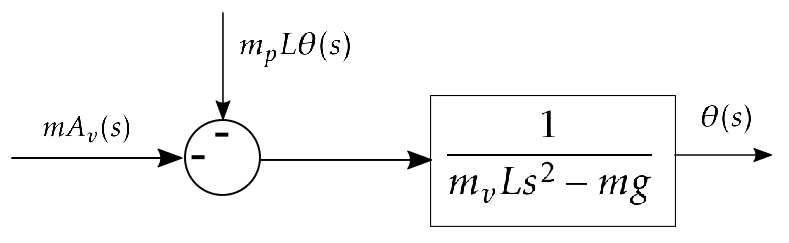
\includegraphics[width=.6\textwidth]{billeder/pendul_trans1.png}
	\caption[Model af overførelsesfunktion for vogn og pendul.]{Model af overførelsesfunktion for vogn og pendul fra ligning \ref{eq:pendul_final}.}
	\label{fig:pendul_trans1}
\end{figure}
\FloatBlock

I overførelsesfunktionen for pendulet indgår massen for vognen $m_v$ og den samlede masse for systemet $m = m_v + m_p$.
Da der ønskes at forsimple pendulets overførelsesfunktion antagess der, at massen af pendulet er lille i forhold til massen af vognen. 
Der kan således lave approksimationen $m \approx m_v$ og der fås således
\begin{align}
\frac{1}{m_vLs^2 - mg } \approx  \frac{1}{m \left( Ls^2 - g \right) } 
\end{align}     
\husk{fraannk}{således}
Modellen i figur \ref{fig:pendul_trans1} kan nu forenkles yderligere, hvorved masserne næsten udgår af systemet.
Den eneste tilbageblivende masse, er for forstyrrelsen på pendulstangen, der ender som $m_pL\theta(s) \approx  \frac{m_p}{m_v}L\theta(s) $.

\begin{figure}[h!]
	\centering
	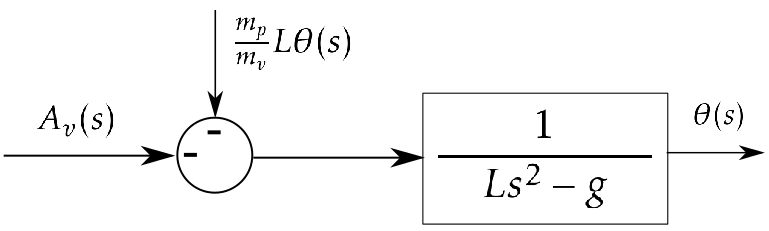
\includegraphics[width=.6\textwidth]{billeder/pendul_trans_clean.png}
	\caption{Simplificeret model af overførelsesfunktion for vogn og pendul.}
	\label{fig:pendul_trans_clean}
\end{figure}
\FloatBlock 
Således endes der med en model (figur \ref{fig:pendul_trans_clean}) af pendulet, der relaterer en påført acceleration $A_v(s)$ til en ændring af vinklen $\theta(s)$

\section{Analyse af vognens overførelsesfunktion}\label{sec:sec_motoroverforelse}

Noter, fremgangsmåde:\\
\begin{itemize}
	\item Måling af a(t) af bilen ved fastsatte I og V=6V
	\item Antagelse af konstant acceleration
	\item Graf af s(t) position som funktion af tiden for fastsatte I
	\item for lav I = ingen acceleration, for høj I = hjulspind
	\item Eftervise antagelsen 
	\item Graf af $\dfrac{ds(t)}{dt}$ og $\dfrac{d^2s(t)}{dt^2} = a(t)$
	\item Plot $I(a)$, Strøm som funktion af acceleration.
	\item Fit -> lineær $I(a) = p_1 a + p_2$
	\item Model af motor $\frac{I(s)}{X(s)}$
	\item Appendiks matlab kode
\end{itemize}


%---------- Chapter ----------------
\chapter{Sensor}\label{kap:chap_sensor}

\emph{I dette kapitel}

%---------- Parts ----------------
\section{Lineær spændingsregulator}\label{sec:lm317}
For at få en konstant spænding på 14\si{\volt} til frekvensgeneratoren, anvendes en LM317. Den har den fordel, at outputspændningen kan styres med kun to modstande.

\husk{Kenneth}{R18 i stykliste}
\subsection{Opstilling}
\husk{Kenneth}{Billede af LM317}


For at finde de to modstandsværdier anvendes formel \ref{eq:lm317_formel}
\husk{Kenneth}{Reference til datablad(Formel)}

\begin{align}
	V_{out} & = V_{ref} \cdot \left( 1 + \frac{R_3}{R_4} \right) + I_{ADJ} \cdot R_3 \label{eq:lm317_formel}
\end{align}

Hvor $V_{ref} = 1.25\si{\volt}$ og $I_{ADJ} = 100\si{\micro\ampere}$. Indsættes værdierne i formlen fåes en outputspænding på 15\si{\volt}. Grunden til, at spændingen bliver 15\si{\volt} og ikke 14\si{\volt}, er adjust-ledet, $I_{ADJ} \cdot R_3$, som normalt kan negligeres, hvilket ikke er tilfældet her, da modstandsværdierne er for store. Vælges komponentværdierne $R_3 = 3.3\si{\kilo\ohm}$ og $R_4 = 330\si{\ohm}$ fås en outputspænding på 14.08\si{\volt}. Dog vælges der ikke at ændre komponentværdierne, dels fordi de allerede var loddet på printet, og fordi det frekvensgeneratorens maksimale inputspænding er 16\si{\volt}.
\section{Frekvensgenerator}\label{sec:frekv_gen}
I dette afsnit vil alle overvejelser omkring frekvensgeneratoren blive gennemgået, hertil designvalg og beregninger. 
\subsection{Design}
Til at generere et signal ud fra batterierne anvendes en timer-kreds. 
Timeren skal her bruges til at lave et puls-signal, der har en given frekvens og duty-cycle, i dette projekt et firkantsignal. 
Der er her valgt en konfiguration der hedder A-stable. 
Fordelen ved dette er at timeren kan hente sit input direkte fra forsyningen der i dette tilfælde er et batteri. Dette koster en ekstra modstand men har den fordel, at duty-cycle og frekvens bliver frie variabler. 
Dette signal skal have en frekvens, der er tilpas høj, så systemet er mindre modtagelig overfor forstyrrelser, og det vil samtidig give en hurtigere responstid. 

Outputsignalet fra timeren er begrænset således, at udgangsspændingen kun kan antage positive værdier.
For at løse dette, sættes en kondensator i serie med spolen.
Det gør at spolen bliver påtrykt en spænding af varierende polaritet, hvilket også giver et konstant skiftende magnetfelt.
\begin{figure}[h!]
	\centering
	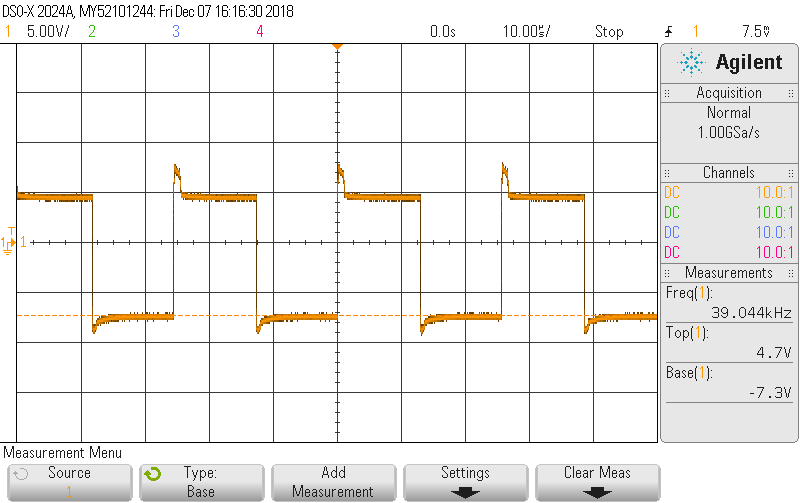
\includegraphics[width=1\textwidth]{billeder/freq_png.png}
	\caption{Her ses outputtet fra frekvensgeneratoren}
	\label{fig:frekvensgenerator}
\end{figure}
Inden kredsløbet tegnes færdigt skal der tages højde for den spænding timeren leverer. 
Spolen har en meget lille indre modstand, hvilket medfører at ved høje spændinger, skal timeren levere en stor strøm. 
Da timeren ikke kan holde til at levere mere end $225 \si{\milli\ampere}$, sættes en modstand i serie for at begrænse strømmen. 
Det færdige kredsløb ses på figur \husk{Kenneth}{indsættelse af figur}

\subsection{Beregninger af komponenter}
Til udregning af modstandens og kondensatorens værdier anvendes to af de ligninger der er opgivet i databladet for NE555 timeren. 
Først anvendes ligning 5 i databladet til at bestemme modstanden $R_5$. 
Da der ikke er ligninger nok, bliver duty-cyclen og modstanden $R_6$ valgt. 
Duty-cyclen sættes til $D = 51\%$  , og $R_6$ vælges til$ 15\si{\kilo\ohm}$. 
Ligning 5 \cite[Side 11.]{NE555} i databladet omskrives svarende til i ligning \ref{eq:TimerInputModstand}.
\begin{align}
R_5 & = \frac{R_6}{D} - 2 \cdot R_6 \label{eq:TimerInputModstand}
\end{align}
Parametrene indsættes i ligning \ref{eq:TimerInputModstand}.
Resultatet viser her at $R_5$ skal være $588\si{\ohm}$ for at opnå en duty-cycle på $51\%$ .
Som det sidste skal der udregnes en kondensator der forbindes til trigger indgangen og til ground. 
Til dette anvendes ligning 4 i databladet \cite[Side 11]{NE555}. Denne ligning isoleres for kondensatoren som givet i ligning \ref{eq:Kondensator_c7}.
Modstandsværdierne er kendte, og der bestemmes her for en frekvens på $F_n = 50 \si{\kilo\hertz}$.
\begin{align}
	C_7 & = \frac{1}{F_n \cdot \left( \frac{25 \cdot R_5 }{36} + \frac{25 \cdot R_6}{18} \right) \label{eq:Kondensator_c7}}
\end{align}
Ud fra ligning \ref{eq:Kondensator_c7} fås en kondensator værdi på $C_7 = \SI{0.9}{\nano\farad}$ for at få en frekvens på 50 \si{\kilo\hertz}. 
Da disse størrelser ikke kan realiseres i de lagerførte SMD værdier, vælges derfor tilnærmede værdier. 
Dette medfører at $R_5$ bliver $680\si{\ohm}$ og $C_7$ på $1\si{\nano\farad}$. 
Heraf udregnes duty-cycle og frekvens ved at bruge ligning 4 og 5 i databladet. \cite[Side 11.]{NE555}

Dette giver en duty-cycle på $D = 49\%$ og en frekvens $F_n = \SI{46.9}{\kilo\hertz}$. 
Duty-cyclen ligger tæt på $50\%$ og den ønskede frekvens er stadig stor nok til at en lille afvigelse ikke kommer til at have en væsentlig betydning. Denne opstilling accepteres.

Der skal herefter sættes en kondensator på udgangen, således at udgangsspændingen kan antage både positive og negative værdier. 
Middelspændingen over en spole er $0\si{\volt}$, men det er outputtet ikke, da den ikke oscillerer omkring $0 \si{\volt}$, hvilket er kondensatorens formål. 
\subsection{Beregning af udgangskondensator}
For at kunne finde afsenderspolens impedans, anvendes vinkelfrekvensen $\omega_c$ som udregnes i ligning \ref{eq:vinkelfrekvens}.
\begin{align}
	\omega_c & = 2 \cdot \pi \cdot F_n \label{eq:vinkelfrekvens}
\end{align}
Der fås en vinkelfrekvens på $\omega_c = \SI{294.91}{\kilo\radian\per\second}$.
Afsenderspolens induktans måles ved hjælp af en RLC-meter til $L = 205\si{\micro \henry}$.
Det ønskes ikke at spolens impedans bliver lige så stor som kondensatorens, idet der så opstår en resonanskreds. 
Spolens impedans udregnes ved ligning \ref{eq:impedans2}.

Den udregnede impedans er $Z_L = \SI{60.5}{\ohm}$.
Der vælges her at spolens impedans skal være 20 gange større end kondensatorens impedans. Størrelsen på kondensatoren udregnes ved ligningen \ref{eq:kondensator_c9}.
\begin{align}
	Z_{C9} & = \frac{20}{\omega_c \cdot C_9} \rightarrow C_9 = \SI{1.1}{\micro\farad} \label{eq:kondensator_c9}
\end{align}
Ved en kondensator størrelse på $C_9 = \SI{1.1}{\micro\farad}$ er størrelsesforholdet mellem de 2 impedanser 20 gange. 
SMD kondensatoren der passer til er på $ 1\si{\micro\farad}$. Det praktiske størrelsesforhold udregnes igen hvor $ 1\si{\micro\farad}$. Størrelsesforholdet bliver da $\si{Z_L \per Z_{C9}} = \num{17.8}$ gange, hvilket er acceptabelt.

På grund af modstanden og kondensatoren i kredsløbet, opstår der en forsinkelse i systemet, der er lig produktet af kondensatoren $C_9$ og modstanden $R_7$. $R_7$ er et potentiometer, så i beregningen anvendes højeste værdi, som er $1\si{\kilo\ohm}$.
\begin{align}
	\tau & = R \cdot C = 1 \si{\milli\second}
\end{align}
Forsinkelsen på $1 \si{\milli\second}$ er acceptabelt for systemet.


\section{Design af spoler}\label{sec:sec_spole_design}

Dimensionering af spoler:

Systemet består af 3 spoler. 1 stor spole til at vidergive et signal, og 2 mindre spoler med samme areal til at opfange et signal. Dimensioneringen afhænger af størrelserne på spolerne. Der er nogle fysiske pladskrav, som begrænser dimensioneringen. Som udgangspunkt, dimensioneres den store spole først, som skal sende et signal videre. (omformuler blot udkast..)

Figur her!!

 \begin{alignat}{3}
 	&\vec{r'}=R(cos(\phi)\hat{i}+sin(\phi)\hat{j})
 \end{alignat}

\begin{alignat}{3}
	&id\vec{s}=i\frac{d\vec{r'}}{d\phi}=i R d\phi (-sin(\phi)\hat{i}+cos(\phi)\hat{j})
\end{alignat}
Stedvektor:
\begin{alignat}{3}
	&\vec{r_p}=z\hat{k}
\end{alignat}

relativ stedvektor
\begin{alignat}{3}
	&\vec{r}=\vec{r_p}-\vec{r'}=-R cos(\phi)\hat{i}-sin(\phi)\hat{j}+z\hat{k}
\end{alignat}

Biot-savarts lov:
\begin{alignat}{3}
	&d\vec{B}=\frac{\mu_0  i}{4\pi} \frac{d\vec{s} \times \hat{r}}{r^2}
\end{alignat}

\begin{alignat}{3}
	&\hat{r}=\frac{\vec{r}}{r}
\end{alignat}

\begin{alignat}{3}
	&r= \mid \vec{r} \mid = \sqrt{R^2+z^2}=\mid \vec{r_p}-\vec{r'} \mid
\end{alignat}



ganger igennem med ovenstående. (ligning?)

\begin{alignat}{3}
	&d\vec{B}=\frac{\mu_0 i}{4\pi} \frac{d\vec{s} \times \vec{r}}{r^3}
\end{alignat}

	
\begin{alignat}{3}
	&d\vec{s}\times(\vec{r_p}-\vec{r'})=R d\phi (-sin(\phi)\hat{i}+cos(\phi)\hat{j})\times (-R cos(\phi)\hat{i}-sin(\phi)\hat{j}+z\hat{k})
\end{alignat}	
Som yderligere kan reduceres ned til:

\begin{alignat}{3}
	R \phi (z cos(\phi)\hat{i}+z sin(\phi)\hat{j}+R\hat{k})
\end{alignat}

\begin{alignat}{3}
	&d\vec{B}=\frac{\mu_0 i}{4\pi} \frac{d\vec{s}\times (\vec{r_p}-\vec{r'})}{(\sqrt{R^2+z^2})^2}=\frac{\mu_0 i}{4\pi} \frac{R \phi (z cos(\phi)\hat{i}+z sin(\phi)\hat{j}+R\hat{k})}{(R^2+z^2)^\frac{3}{2}}
\end{alignat}


Ud fra dette, kan x og y komposanterne af B feltet sættes til = 0. Dette bevises ud fra:
\begin{alignat}{3}
	&\frac{\mu_0 R z}{4\pi} \int\limits_{0}^{2\pi}cos(\phi)d\phi = 0
\end{alignat}


\begin{alignat}{3}
	&\frac{\mu_0 R z}{4\pi} \int\limits_{0}^{2\pi}sin(\phi)d\phi = 0
\end{alignat}

Herefter er der kun z komposanten tilbage:
\begin{alignat}{3}
	&B=\frac{\mu_0 R z}{4\pi} \int\limits_{0}^{2\pi}d\phi
\end{alignat}

Og dermed et udtryk for B i en cirkel.... (ret tekst her samt alle andre steder ved udledning.):


\begin{alignat}{3}
	&B=\frac{\mu_0 iR^2 2\pi}{2(R^2+z^2)^\frac{3}{2}}
\end{alignat}




Tekst omkring solenoid her samt figur.



\begin{alignat}{3}
	&di=inz'
\end{alignat}

\begin{alignat}{3}
	&n=\frac{N}{L}
\end{alignat}

\begin{alignat}{3}
	&d\vec{B}=\frac{\mu_0 R^2}{2[(z-z')^2+R^2]^\frac{3}{2}}di = \frac{\mu_0 R^2 i n dz'}{2[(z-z')^2+R^2]^\frac{3}{2}}
\end{alignat}


B felt i et givet punkt P centreret ud fra z aksen, med funktion af z er dermed givet ved:
\begin{alignat}{3}
	&B(z)=\frac{\mu_0 n R^2 i}{2}\int\limits_{0}^{2\pi}\frac{1}{2[(z-z')^2+R^2]^\frac{3}{2}}dz'
\end{alignat}

\begin{alignat}{3}
	&B(z)=\frac{\mu_0 n i}{2}\bigg[\frac{\frac{L}{2}-z}{\sqrt{(\frac{z-L}{2})^2+R^2}}+\frac{\frac{L}{2}+z}{\sqrt{(\frac{z+L}{2})^2+R^2}}\bigg]
\end{alignat}



%---------- Chapter ----------------
\chapter{Signal}\label{kap:chap_signal}	

%---------- Parts ----------------
\section{Shunt regulator}\label{sec:shunt}
En shunt regulator er en spændingsregulator der benytter en zenerdiode til at regulere spændings niveauet.
Idet forsyningsbatterierne ikke kan holde en konstant udgangsspænding, kan operationsforstærkerne ved høj forstærkning gå i mætning. 
For at undgå det, anvendes shunt regulatoren, da den kan holde en nogenlunde konstant spænding, på trods af batteriernes faldende udgangsspænding.

\subsection{Design}
\begin{wrapfigure}{r}{0.5\textwidth}
	\centering
	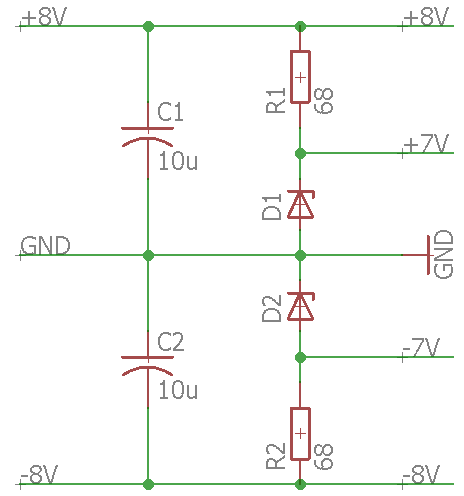
\includegraphics[width=0.48\textwidth]{billeder/shunt_regulator.png}
	\caption{Diagram over shunt regulator}
	\label{fig:ActiveFilter}
\end{wrapfigure}
Der skal her designes en shunt regulator der får $\SI{8.4}{\volt}$ på indgangen, og laver $7\si{\volt}$ på udgangen.
Der bruges to shunt regulatore, idet der forsyningerne til operationsforstærkerne kræver en positiv og en negativ forsyning på 7 \si{\volt}.

\begin{figure}[h!]
	\centering
	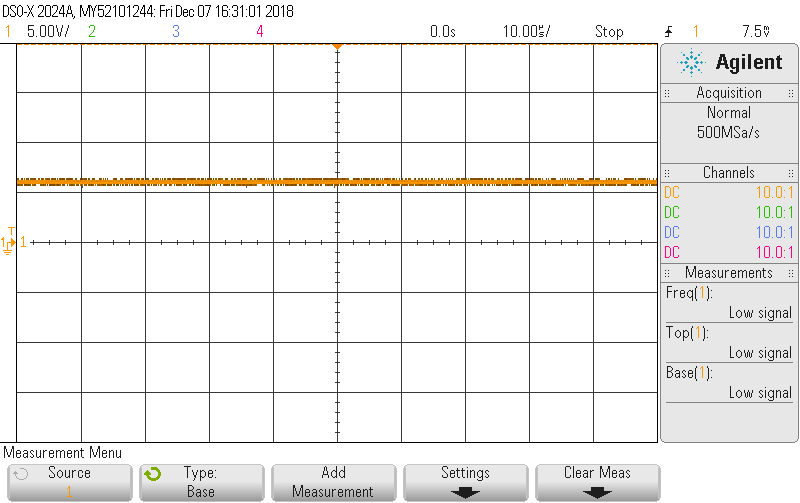
\includegraphics[width=1\textwidth]{billeder/shunt_pos_png.png}
	\caption{Her ses outputtet fra den positive shunt regulator}
	\label{fig:positiv_shunt}
\end{figure}
\subsection{Beregninger}
Indgangsspændingen fra batterierne er $V_{in} = \pm \SI{8.4}{\volt}$. 
For at overskueligegøre beregningerne, anvendes kun den positive spænding, hvoraf komponentværdierne antager samme værdi for den negative spænding, dog bliver zenerdioden forspændt i modsat retning.
Udgangsspændingen ønskes at $V_{out} = 7 \si{\volt}$. 
Indgangsstrømmen vælges til $I_{in} = 20\si{\milli\ampere}$, og bruges til at bestemme udgangsstrømmen.
Zenerdiodens strøm og modstand findes i databladet $I_Z = 5 \si{\milli\ampere}$ $r_z = 15 \si{\ohm}$. \cite[Side. 1 Kolonne 12]{ZenerDiode}

For at der skal ligge en konstant spænding på $7 \si{\volt}$ udregnes først breakdown spændingen over dioden ved at bruge formel \ref{eq:BreakdownVolt} \cite[Side. 146]{Sedra19uu} formlen for spændingen over dioden er den samme som udgangsspændingen på loaden. 
\begin{align}
	V_o & = V_{Z0} + r_z I_z \label{eq:BreakdownVolt} \\
	V_{Z0} & = \SI{6.925}{\volt}
	\end{align}
Værdien $V_{Z0}$ er diodens breakdown spænding.
Breakdown er det punkt hvori spændingsfaldet over dioden er konstant og bliver anvendt til at få en konstant udgangsspænding.
For at beregne modstanden anvendes ligning \ref{eq:RegulatorModstand} \cite[Side. 149]{Sedra19uu}.
\begin{align}
	R_1 & = \frac{V_{in}-V_{Z0}-r_z I_z}{I_z+I_{out}} = 70\si{\ohm} \label{eq:RegulatorModstand}
\end{align}
Modstanden udregnes til $70 \si{\ohm}$, hvoraf den tilnærmede værdi bliver $R_1 = 68 \si{\ohm}$.
Til dette anvendes ligning \ref{eq:UdgangShunt} \cite[Side. 149]{Sedra19uu}.
\begin{align}
	V_{out} & = V_{Z0} \cdot \left( \frac{R_1}{R_1+r_z} \right) + V_{in} \cdot \left( \frac{r_z}{R_1+r_z} \right) - I_{out} \cdot \left( \frac{r_z \cdot R_1}{r_z+R_1} \right) \label{eq:UdgangShunt}
\end{align}
Udgangsspændningen bliver da $V_{out} = \SI{7.04}{\volt}$.

Ovenstående beregninger er udført for en BZX79C6V8 diode. 
Da der blev lavet en endelig komponentliste blev der ved et uheld valgt en BZX79C6V2 diode i stedet for. 
Forskellen her er at den nye diode maksimalt kan holde en konstant spænding på $\SI{6.6}{\volt}$ i udgangsspænding og diode modstanden er $r_z = 10 \si{\ohm}$ \cite[Side. 1 Kolonne 11]{ZenerDiode}.
Ved tilsvarende udregninger findes det frem til at udgangsspændingen er $\SI{6.66}{\volt}$ ved en modstand på $68 \si{\ohm}$.

\section{Båndpassfilter}\label{sec:filter}
Til at fjerne støj og andre udefrakommende forstyrrelser i systemet, skal der laves et filter.
Der vil her blive designet et aktivt båndpas filter, da der kun ønskes at én bestemt frekvens forstærkes.
Fordelen ved det aktive filter er at den kan både forstærke og filtrere.

\subsection{Design}
\begin{wrapfigure}{r}{0.5\textwidth}
	\centering
	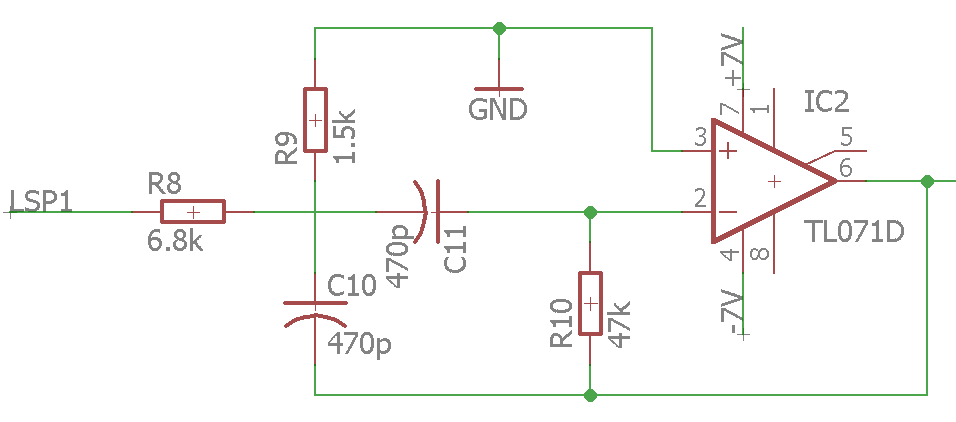
\includegraphics[width=0.48\textwidth]{billeder/ActiveFilter.png}
	\caption{Diagrammet er en repræsentativ tegning \cite[Side. 208]{Huelsman1993}}
	\label{fig:ActiveFilter}
\end{wrapfigure}
Opstillingen af filteret ses på figur \ref{fig:ActiveFilter}.
Filteret er designet så modstanden $R_5$ gør forstærkningen ved resonansfrekvens til en fri variable.
Heraf designes filteret efter en ønsket båndbredde, resonansfrekvens og resonansfrekvens forstærkning. Q er systemets godhed og anvendes til at bestemme bredden på båndbredden. 
$f_0$ er resonansfrekvensen der bestemmer ved hvilken frekvens filterets maksimale forstærkning optræder.
$H_o$ er forstærkningen ved den ønskede centerfrekvens.
\subsection{Beregninger}
For at udregne modstandsværdier skal der vælges størrelse på kondensatorene, forstærkning ved resonansfrekvens og filterets godhed.
Det er her besluttet at begge kondensatorer skal være lige store for at simplificerer udregningerne.
Kondensatoren vælges til $C_{10} = 470 \si{\pico\farad}$, godheden vælges til $Q_g = 3$, resonansfrekvens forstærkingen vælges til $H_o = 3$ og resonansfrekvensen vælges til samme frekvens som på udgangen af timeren, $f_0 = \SI{46.936}{\kilo\hertz}$.
Heraf udregnes båndbredden for filteret og filtermodstandene \cite[Side. 209]{Huelsman1993}.
Til udregning af resonansvinkelfrekvensen henvises til ligning \ref{eq:vinkelfrekvens}.
\begin{align}
	B_w & = \frac{f_0}{Q_g}
	\end{align}
Filterets båndbredde er givet ved forholdet mellem resonansfrekvensen og filterets godhed.
\begin{align}
	R_8 & = \frac{Q_g}{\omega_c \cdot C_{10} \cdot H_o } \label{eq:R8}
	\end{align}
Filterets indgangsmodstand er med til at påvirke systemets centerfrekvens forstærkning, men den kan ikke alene gøre den til en fri variable. 
\begin{align}
	R_9 & = \frac{Q_g}{ \omega_c \cdot C_{10} \cdot \left( 2 \cdot Q_g^2 - H_o \right) } \label{eq:R9}
	\end{align}
Modstanden $R_9$ er med til at gøre forstærkningen til en fri variabel, hvis denne ikke var med, så havde filterets forstærkning været afhængig af godheden.
\begin{align}
	R_{10} & = \frac{2 \cdot Q_g}{ \omega_c \cdot C} \label{eq:R10}
\end{align}
Feedback modstanden regnes ved ligning \ref{eq:R10}.
Dette medfører. $R_8 = \SI{7.215}{\kilo\ohm}$, $R_9 = \SI{1.430}{\kilo\ohm}$, $R_{10} = \SI{43.288}{\kilo\ohm}$ og $B_w = \SI{15.645}{\kilo\hertz}$.
Da disse modstands værdier ikke kan realiseres i SMD, vælges derfor tilnærmede størrelser.
De tilnærmede komponentværdier kommer til at være. $R_8 = \SI{6.8}{\kilo\ohm}$, $R_9 = \SI{1.5}{\kilo\ohm}$ og $R_{10} = 47 \si{\kilo\ohm}$.
De tilpassede komponenter medfører at systemet har en anden karakteristik end den udregnede. 
Til udregning anvendes ligningerne 13a, 13b og 13c \cite[Side. 208]{Huelsman1993}. 
\begin{align}
	f_0 & = \frac{\sqrt{1+\frac{R_9}{R_8}}}{\left( 2 \cdot \pi \right) \cdot \sqrt{R_9 \cdot R_{10} \cdot C_{10}^2}}
	\end{align}
Centerfrekvensen ændrer sig hvis de teoretiske værdier ikke kan opfyldes. Denne ligning bruges til at udregne hvor den nye centerfrekvens kommer til at ligge.
\begin{align}
	Q_g & = \left( \frac{2 \cdot \sqrt{\frac{R_9 \cdot C_{10}}{R_{10} \cdot C_{10}}}}{\sqrt{1+\frac{R_9}{R_8}}} \right)^{-1}
	\end{align}
Når kondensatorene er lige store så har de ingen indflydelse på filterets godhed. Denne ligning er kun afhængig af modstandsværdierne i dette tilfælde.
\begin{align}
	H_o & = \frac{\frac{R_{10}}{R_8}}{1+\frac{C_{10}}{C_{10}}}
\end{align}
Tilsvarende for godheden så har kondensatorene ikke nogen påvirkning når de er lige store.
Ændringen er her udelukkende afhængig af indgangs og feedback modstand.
Dette medfører at systemets karakteristik er. 
$H_o = \num{3.5}$, $f_0 = \SI{44.557}{\kilo\hertz}$, $Q_g = \num{3.1}$ og $B_w = \SI{14.4}{\kilo\hertz}$. 
En forøgelse på $16 \%$ på forstærkningen kommer ikke til at blive et problem så længe instrumenterings forstærkeren ikke går i mætning. 
Centerfrekvens ændringen er acceptabel, da den ikke ligger så langt fra den teoretiske at det forårsager den dæmpning af spændingen.
En højere godhed medfører at båndbredden bliver mindre, men da båndbredden stadig er stor, så kommer det ikke til at gøre systemet signifikant langsommere.
\begin{figure}[h!]
	\centering
	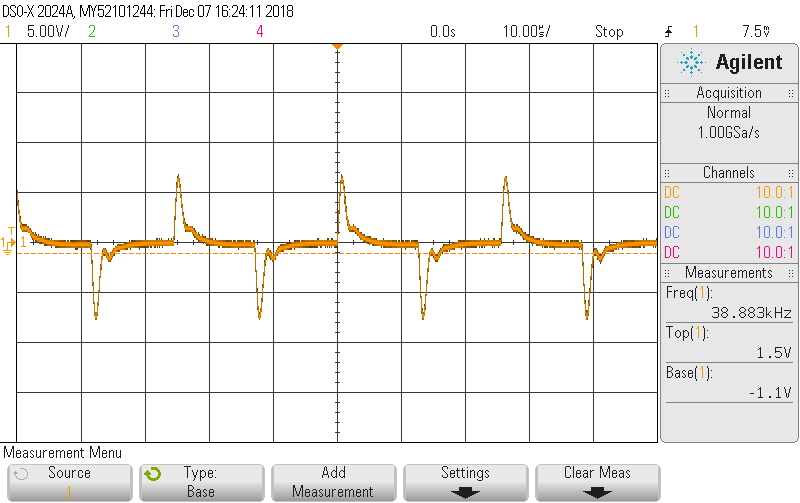
\includegraphics[width=1\textwidth]{billeder/filter_in_png.png}
	\caption{Her ses signalet fra modtagerspolen før filteret.}
	\label{fig:filter_in}
\end{figure}
\begin{figure}[h!]
	\centering
	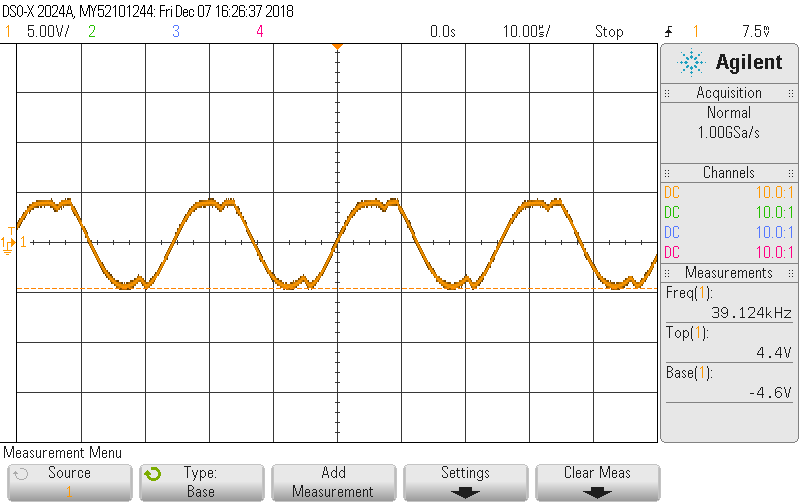
\includegraphics[width=1\textwidth]{billeder/filter_out_png.png}
	\caption{Her ses signalet efter filteret, hvor signalet er forstærket i filteret.}
	\label{fig:filter_out}
\end{figure}
\section{Ensretter}\label{sec:ensretter}
\husk{Kenneth}{Billede af output fra ensretter}
Da modtagerspolerne får overført signalet der genereres af frekvensgeneratoren, så vil inputtet til instrumenteringsforstærkeren få en tilnærmet sinus. 
For at undgå det, anvendes en ensretter kreds, for at få et konstant signal.

\subsection{Design}
Enretteren består af en diode, forspændt i lederetningen, der er koblet serielt med en parallelkobling af en spole og en modstand. 
Diodens funktion er at lade halvdelen af signalet passere, hvilket betyder at signalets negative del frafalder. 
For ikke at få et variende positivt pulssignal, indsættes kondensatoren for at glatte spændingen ud. Modstandens funktion er at aflade kondensatoren, så


\husk{Kenneth}{Billede af ensretter kredsløb} 

\subsection{Beregninger}
Til udregning af komponentværdier til ensretteren, antages at en peak spænding på 2 volt.

\begin{align}
	V & = 2 \si{\volt} \nonumber
\end{align}

Der vælges en rippelspænding på 15\% af peakspændingen
\begin{align}
	V_{rip} & = 300 \si{\milli\volt} \nonumber
\end{align}
Da der ikke er ligninger nok til at bestemme alle variable, bestemmes afladningsmodstaden til
\begin{align}
	R_{11} & = 5 \si{\kilo\ohm} \nonumber
\end{align}
Modstanden og kondensatoren sidder parallelt, hvilket gør at strømmen gennem kondensatoren kan beregnes ved Ohm's lov. Denne strøm bruges både til opladning og afladning.
\begin{align}
	i & = \frac{V}{R_{11}} \\
	i & = 400 \si{\mu\ampere}\nonumber
\end{align}

Den teoretiske værdi for kondensatoren udregnes ved hjælp af ligning 3.36 i bog "\cite[side. 160]{Sedra19uu}".
\begin{align}
	C_{14} & = \frac{V}{V_{rip} \cdot F_c \cdot R_{11}}\\
	C_{14} & = 30nF \nonumber
\end{align}


På grund af komponentværdi begræsninger i SMD rækken (E6) på komponentlageret, vælges afladningsmodstanden $R_{11} = 4.7 \si{\kilo\ohm}$, hvoraf en ny teoretisk kondensatorværdi findes $C_{14} = 22 \si{\nano\farad}$.


$\tau$ er tidskonstanten mellem modstanden og kondensatoren, og er forsinkelsen mellem opladning og afladningen. 
\begin{align}
	\tau & = C_{14} \cdot R_{11}
\end{align}

Da signalet skal ensrettes, skal tidskonstanten, $\tau$ være meget større end periodetiden $T = \frac{1}{F_c}$, for at glatte signalet ud. Periodetiden udregnes til $T = 22 \si{\micro\second}$.
\begin{align}
	\tau & \gg T \nonumber
\end{align}
Vælges en kondensatorværdi på $C_{14} = 100 \si{\nano\farad}$ fås et forhold på,

\begin{align}
	\frac{\tau}{T} & = 21
\end{align}
hvilket svarer til at afladningstiden er 21 gange større end periodetiden. Det er sikre en lille ripplespænding, så er udgangsspændingen tilnærmelsesvis en DC.
\section{Instrumenteringsforstærker}\label{sec:summa}
\husk{Kenneth}{Billede af output fra instrumenteringsforstæker}
For at få en retning ud af spolesignalerne, anvendes instrumenteringsforstærkeren AD623. Instrumenteringsforstærkeren er valgt frem andre operationsforstærker typer, da den har meget større indgangsimpedans, hvilket er hensigtsmæssigt, da strømmene fra modtagerspolerne ikke er særligt store. Valget af instrumenteringsforstærkeren har også den fordel, at forstærkningen kan styres med blot en modstand, hvilket sparer plads på print boardet.


\subsection{Design}
Det samlede kredsløb for instrumenteringsforstærkeren består af en AD623, en gain modstand, samt et potentiometer. Dertil er der påsat to afkoblingskondensatorer. Kredsen forsynes med +- 7 volt, da det er max output fra batterierne. 

\husk{Kenneth}{Billede af instrumenterings kredsløb} 

\subsection{Beregninger}
\husk{Kenneth}{Find ud af spændingen før forstærkning. Også i filteret}
Da indgangssignalerne til instrumenteringsforstærkeren er meget lave, anvendes en gainmodstand for at forstærke signalet.

Der tilstræbes en forstærkning på 4 - 5 gange. Forstærkningen udregnes med ligning \ref{eq:GainModstand}.
\begin{align}
	R_G & = \frac{100 \si{\kilo\ohm}}{G-1} \label{eq:GainModstand}
\end{align}
hvor en gainmodstand på 22 \si{\kilo\ohm} giver en forstærkning på 4.5.
\husk{Kenneth}{Husk gain tabel i bilag} 
\section{Delkonklusion af signalbehandling}\label{sec:delkonklusion_signal}

%---------- Chapter ----------------
\chapter{Motorstyring og reguleringssystem}\label{chap:motor_reg}

\emph{Udgangssignalet fra sensor systemet skal medføre en bevægelse af vognen, således at pendulstangen forbliver oprejststående. I Dette kapitel vil motorstyringen blive dimensioneret og udarbejdet, som gør bevægelse af vognen mulig. Til sidst vil det vigtige reguleringssystem nu dimensioneres. }

%---------- Parts ----------------
\section{Motorstyring }\label{sec:sec_motorstyring}
Målinger af vognens dynamik gennemgået i afsnit \ref{sec:sec_motoroverforelse}, er baseret på stepresponset af vognen ved en konstant spænding, men med faste strømbegrænsninger i intervaller.

Dette giver anledning til at vægle en motorstyring der sørger for en konstant strøm til motoren.
 
Således vil udgangssignalet fra regulatoren i form af en reguleringsspænding, $V_{reg}$ omsættes i motorstyringen til den ønskede strøm $I_{reg}$, der igen giver den ønskede acceleration af vognen.  


\begin{itemize}
	\item Omsætter volt til ampere (current control)
	\item Pnp og npn transistorer med relativ høj strømrate
	\item Motor accelererer baseret på ampere. Volt angiver tophastighed.
	\item Min 1.25A maks 2.25A
\end{itemize}

\subsection{Design og dimensionering af motorregulering}
\husk{Kenneth}{Tekst rettes}
Da DC-motoren er en kompleks enhed, hvis dynamik og opbygning ligger uden for opfanget af denne rapport. 
Anvendes en simpel feedback regulering af strømmen igennem transistorerne, således at forholdet mellem indgangs signalet og udgangsstrømmen til motoren holdes konstant, som kan beskrives ved
\husk{JJ}{teoretisk model for motor styring}

I fig xx ses den valgte typografi af motor regulator.
\husk{JJ}{Diagram af motorstyring}

\husk{JJ}{Beskrivelse af motor regulator design} 
\husk{JJ}{Håndtering af transiente spændinger igennem bypass dioder}

\subsection{Beregninger}
\husk{JJ}{beregninger af forhold mellem spænding og strøm i regulatoren}
\husk{JJ}{PSpice simulering af regulator}

\subsection{Overførelsesfunktion af motor}
For at bestemme dynamikken af DC-motoren opstilles en forenklet model af motoren.

\begin{figure}[h!]
	\centering
	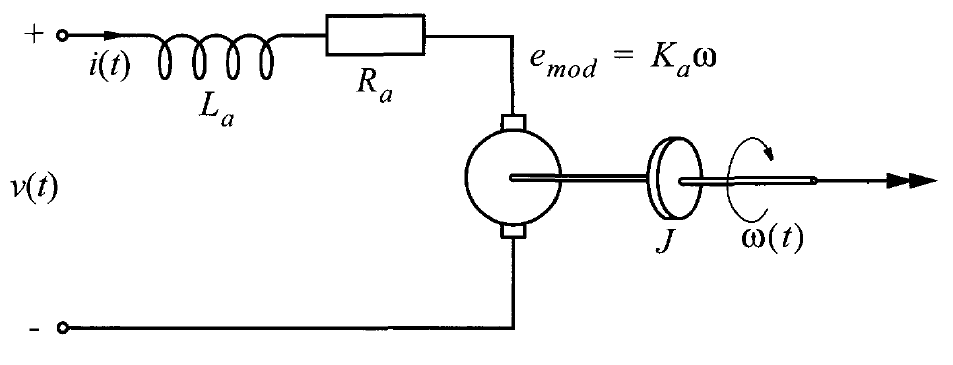
\includegraphics[width=.6\textwidth]{billeder/motor_model.png}
	\caption[sss]{Model af elektromotorisk system til brug ved modellering af motor\protect\footnotemark.}
	\label{fig:motor_model}
\end{figure}
\FloatBlock
\footnotetext{Figuren er tilrettet fra \cite[Figur 2.16, s. 52]{Reg2015}}

Ved at fastholde motoren, således at den mod-elektromotoriskekraft ($e_{mod}$) kan sættes til nul dvs. $\omega = 0$, er det muligt at måle motores induktans.
Modellen kan således omstilles som
\begin{align}
	v(t) = R_ai(t) + L_a\dfrac{di(t)}{dt}
\end{align}
Måling af strømmen igennem motoren er forstaget over en $0,2 \si{\ohm}$ test-modstand
\footnote{Modstand med meget lille induktans}.
Motorens egen modstand er målt til $R_{motor} = 3,2 \si{\ohm}$, hvilket giver en samlet modstand på $R_a = R_{test} + R_{motor} = 3,4 \si{\ohm}$ i test opstillingen. 

\begin{figure}[h!]
	\centering
	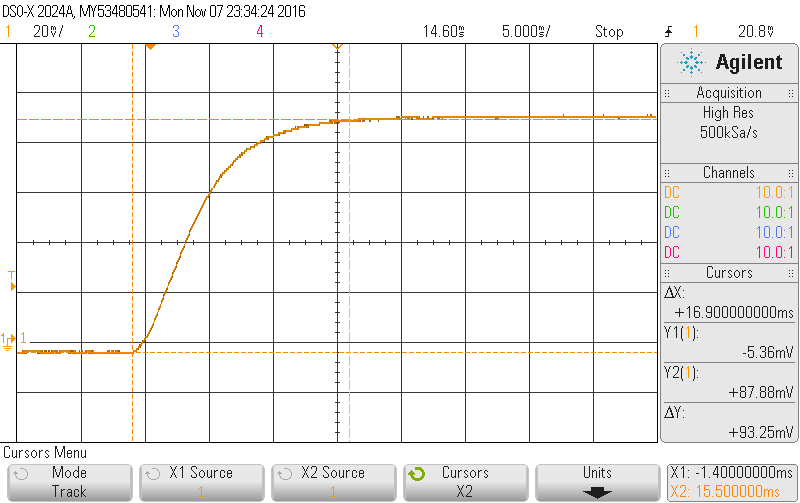
\includegraphics[width=.8\textwidth]{billeder/motor_L.png}
	\caption{Måling af transient forløb for strømmen igennem DC-motor.}
	\label{fig:motor_dynamik_scoop}
\end{figure}


Tidskonstanten for ladning af en spole er, $\tau = \frac{L}{R}$.
For at bestemme $L$, måles tiden $t$ ved $5\tau$ som er ved
\begin{align}
	\% opladning = \left( 1 - \frac{1}{e^{t/\tau}} \right) \cdot 100\% \Rightarrow  \left( 1 - \frac{1}{e^{t/5}} \right) \cdot 100 \approx 99,32\% 
\end{align}
derefter kan $L_a$ bestemmes som, ved aflæst tid på $16,9\si{\milli\second}$ i fig. \ref{fig:motor_dynamik_scoop} 
\begin{align}
	5\tau = \frac{L_a}{R_a} \Rightarrow L_a = 16,9\si{\milli\second} \cdot 3,4 \si{\ohm} = 57,5 \si{\milli\henry}
\end{align}

Overførelsesfunktion for motoren opstilles som
\begin{align}
H_{motor} = \frac{V_o}{V_i} = \frac{s L_a}{s L_a + R_{motor}} = \frac{ \frac{L_a}{R_{motor}}s}{ \frac{L_a}{R_{motor}}s +1} = \frac{\num{18E-3}s}{\num{18E-3}s +1}
\end{align}  



\section{Regulering}\label{sec:regulering}

...
\subsection{Design}

\begin{itemize}
	\item Valg af regulator-type (PD)
	\item Evt. måling af loop gain 
	\item Saturation punkter
	\item Stabilitet
\end{itemize}
....
\subsection{Beregninger}
...



%---------- Chapter ----------------
\chapter{Diskussion og vurdering}\label{kap:diskussion}
Som helhed virkede de fleste af tilgangene for at løfte opgaven tilfredsstillende.
Arbejdsmetoder og workflow viste sig at fungere som forventet.
Planlægning med stramme deadline blev overholdt, og gav anledning til overblik i projektet.

I følgende afsnit vil en mere dybdegående diskussion og vurdering gennemgås med relation til de enkelte afsnit. 

\subsection{Fysisk model}
Ved at anvende klassisk fritlegeme analyse af pendulet lykkedes det at få en reguleringsmæssig brugbar beskrivelse af fysikken. 
Det var dog en lang og besværlig vej at løse problemet på, da man med anden viden, fx Lagrange og statespace analyse ville frembringe et brugbart resultat.
Der blev anvendt en del tilnærmelser i udledningen. 
Da alle tilnærmelser er velargumenteret, vurderes det at deres anvendelse er valide og det endelige resultat anses for korrekt.   

\subsection{Vognens overførelsesfunktioner}
Da hele vognen med pendul og motor var arvet fra en tidligere projekt gruppe, var en af udfordringerne at finde frem til den dynamik der beskriver disse dele.
Den anvendt metode viste sig at fungere og det endelige resultat kunne, ud fra en velovervejet simplificering, anvendes i den samlede systembeskrivelse der ligger til grund for bestemmelsen af regulatoren.
Til fremtidige forbedringer ville udskiftning af fx motor kunne føre til en mere dybdegående beskrivelse af systemets overførelsesfunktion, og derved give en endnu bedre regulering og stabilitet.

\subsection{Sensor}
Ud fra analysering af sammenkoblingen mellem to solenoider, lykkedes det vha. forskellige teorier - heriblandt Faradays lov - at lave en velfungerende model af et sensorsystem. 
Det mest krævende var, at lave et præcist resultat for magnetfeltet, da dette krævede flere teknikker, heriblandt mange matematiske udledninger.
Faktorerne for den inducerede afsenderspole, var meget diskuteret, da strømmen fra frekvensgeneratoren afhang af styrken på magnetfeltet denne dannede - herudover også trådtykkelse og længde. 
Da alle teoretiske beregninger blev eftervist i laboratoriet, antages der med nogen tilnærmelse, at de endelige resultater kan antages for korrekte.\\
Under designet af CAD-tegningerne var det en udfordring at lave et system med nem montering på den arvede vogn. Efter nogle 3D-print forsøg og adskillige målinger lykkedes det at lave et godt brugbart system som var nemt at montere, samt nemt at vikle spoler på. Derudover gav det køretøjet et nogenlunde stilrent udseende, pga. print-monteringspladen og batteri-hus kombinationen.\\
Til dimensionering af timer-kredsen, blev der anvendt vedlagte ligninger i databladet.
Det var herfra muligt at dimensionere komponentstørrelser, der ville lave et signal med en frekvens, der lå tæt på den ønskede.
Desværre viste målinger på kredsløbet, at frekvensen varierede mere på det endelige produkt, end ved breadboard prototypen.
Dette blev først opdaget hen mod slutning af projektet, så fejlfinding ikke var mulig, men fejlen skyldes højst sandsynligt en forkert komponent.
Endvidere viste det sig, at udgangssignalet ikke oscillerede mellem en konstant positiv og negativ spænding af samme størrelse, hvor årsagen til dette er endnu ikke kendt.
En mulig forbedring kunne være at designe en frekvensgenerator baseret på en anden topologi.

\subsection{Signalbehandling}
Ud fra løbende test af hvert kredsløb på breadboards, blev de endelige kredsløb dimensioneret.
På trods af støj i breadboards, virkede kredsløbene efter hensigten.
For at undgå støj i de endelige kredsløb, blev der tilføjet afkoblingskondensatorer, hvor det var muligt.
En mulig forbedring af signalbehandlingen blev undersøgt, hvor der blandt andet blev kigget på en aktiv ensretter kreds. Problemet med denne var dog, at der skulle bruges to operationsforstærkere til én ensretter.
Det endelige kredsløb indeholder to aktiv båndpas filtre, hvilket kunne viste sig at være en god idé, da disse ikke har særlig stor impedans påvirkning af de omkringliggende kredsløb.
Grundet approksimering af komponentværdier til E12 og E6 serien, kom der afvigelser fra de teoretiske forventninger.

\subsection{Motorstyring}
Det viste sig tilstrækkeligt at anvende bi-directional DC-motor driver topologi som styring af motoren. 
Den negative feedback sørgede for en velfungerende regulering af strømmen igennem motoren, som var vigtig for at reguleringssystemet kunne fungere og give den ønskede stabilitet.
Kompleksiteten omkring motoren var stor, så derfor var mange tilnærmelser nødvendige.
Disse tilnærmelser anses dog for at være velbegrundede, men om deres omfang var dækkende, vides dog ikke med sikkerhed.
Under projektarbejdet, viste en manglende strøm igennem motoren at være et problem mht. respons hastigheden af vognen overfor udefrakommende forstyrrelser.     
En ændring af design, der ved indførelse af en ekstra $\pm 9 \si{\volt}dc$ forsyning til motorstyringens operationsforstærker, blev løst.
Det ville på sigt, give en bedre stabilitet at udskifte den nuværende motorstyring, med en der kan håndtere mere effekt, men siden den nuværende motoreffekt giver anledning til mistet vejgreb fra hjul til underlag, vil en opgradering af hjul være et bedre valg. 

\subsection{Regulering}
Opstilling af det samlede reguleringssystem viste sig at være en stor og kompleks opgave.
Der var mange del overførelsesfunktioner der ikke blot skulle beskrives, men det var også nødvendigt at identificere hvilke simplificeringer og lineariseringer der var mulige at lave, uden at miste den nødvendige information i åben-løkke beskrivelsen af reguleringssløjfe.
Valget af P-lead kompensator som regulator viste sige at være tilstrækkeligt og gav den nødvendige fasemargin der skulle til for at stabilisere pendulet.
Det viste sig svært at få målt systemets overførelsesfunktion, men med lidt god vilje ligger målingen rimelig tæt på den teoretiske model. 



							

%---------- Chapter ----------------
\chapter{Konklusion} \label{kap:konklusion}
En klassisk modelfremstilling af det fysiske system kunne give den nødvendige model til at beskrive det inverterede pendul.
Det viste sig muligt, at ved måling og beregninger, at bestemme dynamikken for vogn og motor.
Sammen med overførelsesfunktionerne fra de elektriske kredse i systemet, var det muligt at danne et samlet reguleringssystem og ved klassisk reguleringsteori at fremstille og dimensionere en P-lead regulator, der kunne stabilisere systemet.
Det blev vist at pendulets vinkel kan bestemmes, ved at anvende elektromagnetiske felter frembragt af spoler, hvor der blev opstillet en tilnærmet teoretisk model, der kunne eftervises.
Det blev også eftervist, hvordan magnetiske felter kobler sig imellem 2 spoler.
I det elektriske kredsløb viste en signalbehandling i form af et filter, en ensretning og signalsammenligning sig tilstrækkeligt for at kunne bruge transducerens signal til regulering.
Den valgte motorstyring blev designet så vognen kunne bevæge sig efter hensigten.
Den nødvendige forsyning, til de enkelte kredsløb, kunne med en spændingsregulator og en shunt-regulator realiseres.
Alle nødvendige konstruktionsdele til vognen, kunne med fordel fremstilles ved CAM og 3D-printer teknologi.

Det kan derfor konkluderes at alle punkterne i problemstillingen er blevet besvaret, at det udarbejdede produkt er funktionelt samt overholder de stillede krav for projektet. 							


\SingleSpacing

\nocite{*}
\bibliography{rapport}\label{bilag:litteratur}
\listoffigures
\listoftables

%--------- Bilag -------------------
\appendix
\chapter{Ordliste} \label{bilag:ordliste}

\begin{table}[h!]
	\centering
	\caption{Ordliste}
	\label{tab:ordliste}
	\begin{threeparttable}
		\begin{tabular}{l l}
			\toprule
			\multicolumn{1}{l}{Symbol}       &
			\multicolumn{1}{l}{Beskrivelse}  \\ 
			\midrule
			$A$					& Areal ja hallo en to tre fyldetekst hvor bred bliver vi lorem ipsum LUL PogChamp		\\
			$f$					& Frekvens		\\
			$f_0$				& Resonansfrekvens \\
			$F_g$				& Tyngdekraft	\\
			$P_{m}$				& Fasemargin	\\
			$i$\tnote{*}		& $\sqrt{-1}$ imaginær tal	\\
			$\vec{J}$			& Strømtæthed	\\
			$m$			  		& Masse \\
			$t$			  		& Tid \\
			$Q$					& Ladning \\
			$R$					& Resistans \\
			$P$					& Effekt \\
			$\omega_{c}$		& Krydsfrekvens	\\
			$D*$				& Duty-cycle\\
			$F_c$				& Timerfrekvens\\
			$B_w$				& Båndbredde\\
			$Q_g*$				& Godhed\\
			$H_o*$				& Resonansforstærkning\\
			$V_{Z0}$			& Breakdown spænding\\
			$I_z$				& Diode strøm\\
			$r_z$				& Diode modstands\\
			$T$					& Periode tid\\
			$\tau$				& Tidskonstant\\
			$R_G$				& Gain-modstands\\
			
			\bottomrule
		\end{tabular}
	\end{threeparttable}
\end{table}
\chapter{Symbolforklaring} \label{bilag:symbol}

\begin{table}[h!]
\centering
\caption{Symbolforklaring}
\label{tab:symboler}
\begin{threeparttable}
\begin{tabular}{l l l}
\toprule
\multicolumn{1}{l}{Symbol}       &
\multicolumn{1}{l}{Enhed}        &
\multicolumn{1}{l}{Beskrivelse}  \\ 
\midrule
$A$					&	[\si{\milli\meter}]			& Areal 		\\
$f$					&	[\si{\hertz}]				& Frekvens		\\
$f_0$				&	[\si{\hertz}] 				& Resonansfrekvens \\
$F_g$				&	[\si{\newton}]				& Tyngdekraft	\\
$P_{m}$				&	[\si{\degree}]				& Fasemargin	\\
$i$\tnote{*}		&								& $\sqrt{-1}$ imaginær tal	\\
$\vec{J}$			&	[\si{\ampere\per\meter\squared}]		& Strømtæthed	\\
$m$			  		&	[\si{\gram}] 				& Masse \\
$t$			  		&	[\si{\second}] 				& Tid \\
$Q$					&	[\si{\coulomb}] 			& Ladning \\
$R$					&	[\si{\ohm}] 				& Resistans \\
$P$					&	[\si{\watt}] 				& Effekt \\
$\omega_{c}$		&	[\si{\radian\per\second}]	& Krydsfrekvens	\\
$D*$				&								& Duty-cycle\\
$F_c$				&	[\si{\per\second}]			& Timerfrekvens\\
$B_w$				&	[\si{\radian\per\second}]	& Båndbredde\\
$Q_g*$				&								& Godhed\\
$H_o*$				&								& Resonansforstærkning\\
$V_{Z0}$			&	[\si{\volt}]				& Breakdown spænding\\
$I_z$				&	[\si{\ampere}]				& Diode strøm\\
$r_z$				&	[\si{\ohm}]					& Diode modstands\\
$T$					&	[\si{\second}]				& Periode tid\\
$\tau$				&	[\si{\second}]				& Tidskonstant\\
$R_G$				&	[\si{\ohm}]					& Gain-modstands\\
$L$					&	[\si{\henry}]				& Induktans\\
$B$					&	[\si{\tesla}]				& Magnetfelt\\
$\Phi$				&	[\si{\weber}]				& Magnetisk flux\\
$\xi$				&	[\si{\volt}]				& Elektromotorisk kraft\\
$\delta$			&	[\si{\m}]					& Strømfortrængning\\
$Z$					&	[\si{\ohm}]					& Impedans\\	
$X$					&	[\si{\ohm}]					& Reaktans\\
$I/i$				&	[\si{\ampere}]				& Strøm\\
\bottomrule
\end{tabular}
\begin{tablenotes}
\item[*] \textit{Værdi uden enhed}
\end{tablenotes}
\end{threeparttable}
\end{table}


%------------------------------- Tabel 2 ---------------------------------


\begin{table}[h!]
\centering
\caption{Symbolforklaring fortsat}
\label{tab:symboler2}
\begin{threeparttable}
\begin{tabular}{l l l}
\toprule
\multicolumn{1}{l}{Symbol}       &
\multicolumn{1}{l}{Enhed}        &
\multicolumn{1}{l}{Beskrivelse}  \\ 
\midrule

Symbol & Enhed & Beskrivelse når der ikke er mere plads på side 1 \\

\midrule
\multicolumn{3}{c}{\textbf{Natur- og materialekonstanter\tnote{**}}}       \\
\midrule
$g$         &	[\si{\meter\per\second^2}]		&	Tyngdeaccelerationen: \num{9,82} \\
$\mu_0$		&	[\si{\henry\per\meter}]			&	Permeabilitet i vakuum: \num{1,257e-6} \\
$\rho$		&	[\si{\ohm\cdot\meter}]			&
Resistivitet i kobber: \num{1,678e-8} \\
\bottomrule
\end{tabular}
\begin{tablenotes}
\item[*] \textit{Værdi uden enhed}
\item[**] \textit{Kilde til værdier \cite{Halliday2014}}
\end{tablenotes}
\end{threeparttable}
\end{table}

\chapter{Styklister} \label{bilag:styklister}
\husk{JJ}{Styklister med ref til alle diagrammer}

\begin{table}[h!]
\small
\centering
\caption{Stykliste for diagram xxx}
\label{tab:udstyr}
\begin{threeparttable}
\begin{tabular}{ l l l l l l l }
\toprule
\multicolumn{1}{l}{\textbf{Komp.}}       &
\multicolumn{1}{l}{\textbf{Værdi}}       &
\multicolumn{1}{l}{\textbf{Type}}       &
\multicolumn{1}{l}{\textbf{Tol.}} &
\multicolumn{1}{l}{\textbf{Klasse}} &
\multicolumn{1}{l}{\textbf{Bemærkning}} &
\multicolumn{1}{l}{\textbf{Type / Lev.}}  \\ 
\hline
R1,R2 & $\SI{68}{\ohm}$			& Keramisk	SMD	& $\pm 1\%$ 		 & $\SI{0.25}{\watt}$	  & 100ppm/\si{\celsius}  & RC12 0805, Phycomp \\
R3 & $\SI{10}{\kilo\ohm}$		& Keramisk	SMD	& $\pm 1\%$ 		 & $\SI{0.25}{\watt}$	  & 100ppm/\si{\celsius}  & RC12 0805, Phycomp \\
R4 & $\SI{1}{\kilo\ohm}$		& Keramisk	SMD	& $\pm 1\%$ 		 & $\SI{0.25}{\watt}$	  & 100ppm/\si{\celsius}  & RC12 0805, Phycomp \\
R5 & $\SI{680}{\ohm}$			& Keramisk	SMD	& $\pm 1\%$ 		 & $\SI{0.25}{\watt}$	  & 100ppm/\si{\celsius}  & RC12 0805, Phycomp \\
R6 & $\SI{15}{\kilo\ohm}$		& Keramisk	SMD	& $\pm 1\%$ 		 & $\SI{0.25}{\watt}$	  & 100ppm/\si{\celsius}  & RC12 0805, Phycomp \\
R7,R17 & $\SI{1}{\kilo\ohm}$		& Potentiometer		& $\pm 10\%$ 		 & $\SI{0.5}{\watt}$	  & 100ppm/\si{\celsius}  & 3296 Square Trimpot, Bourns  \\
R8,R13 & $\SI{6.8}{\kilo\ohm}$		& Keramisk	SMD	& $\pm 1\%$ 		 & $\SI{0.25}{\watt}$	  & 100ppm/\si{\celsius}  & RC12 0805, Phycomp \\
R9,R14 & $\SI{1.5}{\kilo\ohm}$		& Keramisk	SMD	& $\pm 1\%$ 		 & $\SI{0.25}{\watt}$	  & 100ppm/\si{\celsius}  & RC12 0805, Phycomp \\
R10,R15 & $\SI{47}{\kilo\ohm}$		& Keramisk	SMD	& $\pm 1\%$ 		 & $\SI{0.25}{\watt}$	  & 100ppm/\si{\celsius}  & RC12 0805, Phycomp \\
R11,R12,R16 & $\SI{4.7}{\kilo\ohm}$		& Keramisk	SMD	& $\pm 1\%$ 		 & $\SI{0.25}{\watt}$	  & 100ppm/\si{\celsius}  & RC12 0805, Phycomp \\
R18 & $\SI{1.5}{\kilo\ohm}$		& Metalfilm	& $\pm 1\%$ 		 & $\SI{0.6}{\watt}$	  & 50ppm/\si{\celsius}  & MRS25, Philips \\
R40 & $\SI{15}{\kilo\ohm}$ 	& Keramisk SMD 	& $\pm 1\%$			& $\SI{0.25}{\watt}$ 	& 100ppm/\si{\celsius}	& RC12 1206, Phycomp \\
R41 & $\SI{1}{\kilo\ohm}$ 	& Keramisk SMD 	& $\pm 1\%$			& $\SI{0.25}{\watt}$ 	& 100ppm/\si{\celsius}	& RC12 1206, Phycomp \\
R42 & $\SI{330}{\kilo\ohm}$ 	& Keramisk SMD 	& $\pm 1\%$			& $\SI{0.25}{\watt}$ 	& 100ppm/\si{\celsius}	& RC12 1206, Phycomp \\
C1,C2,C4,C6,C20, C40 & $\SI{10}{\micro\farad}$ & Keramisk SMD & $\pm 10\%$ & 50 \si{\volt}  & 15ppm/\si{\celsius} & X7R-serie 1206, Phycomp \\
C3,C5,C12,C13,C14,C15,C18,C19,C21,C22, C41,C42 & $\SI{100}{\nano\farad}$ & Keramisk SMD & $\pm 10\%$ & 50 \si{\volt} & 15ppm/\si{\celsius} & X7R-serie 1206, Phycomp \\
C7 & $\SI{1}{\nano\farad}$ & Keramisk SMD & $\pm 5\%$ & 50 \si{\volt} & 30ppm/\si{\celsius} & NP0-serie 1206, Phycomp \\
C8 & $\SI{10}{\nano\farad}$ & Keramisk SMD & $\pm 5\%$ & 50 \si{\volt} & 30ppm/\si{\celsius} & NP0-serie 0805, Phycomp \\
C9 & $\SI{1}{\micro\farad}$ & Keramisk SMD & $\pm 10\%$ & 50 \si{\volt} & 15ppm/\si{\celsius} & X7R-serie 0805, Phycomp \\
C10,C11,C16,C17 & $\SI{470}{\pico\farad}$ & Keramisk SMD & $\pm 10\%$ & 50 \si{\volt} & 15ppm/\si{\celsius} & X7R-serie 0805, Phycomp \\
D1,D2 & BZX79C6V2 & Zener diode & $\pm 5 \%$ & \SI{0.5}{\watt} & \SI{4}{\milli\watt\per\celsius} & Fairchild Semiconductor \\
D3,D4 & 1N4148 & Ensretter diode & N/A & \SI{0.5}{\watt} & \SI{5}{\milli\watt\per\celsius} & Fairchild Semiconductor \\
D5 & LED grøn 3mm & Grøn lysdiode & N/A & \SI{0.1}{\watt} & N/A & Ukendt \\
IC1 & NE555P & Timerkreds SMD & $V_{cc}= 18 \si{\volt}$ & N/A & 50ppm/\si{\celsius} & Texas Instruments \\
IC2,IC3,IC40 & TL071P & Op. Amp SMD & $V_{cc}=\pm 18 \si{\volt}$ & N/A & \SI{18}{\micro\volt\per\celsius} & Texas Instruments \\
IC4 & AD623AN & Op. Amp SMD & $V_{cc} = 12 \si{\volt}$ & \SI{650}{\milli\watt} & 50ppm/\si{\celsius} & Analog Devices \\
IC5 & LM317T & Spændingsregulator & $V_{o} , V_{i} = 40 \si{\volt}$ & \SI{20}{\watt} & $i_{max} = 1.5 \si{\ampere}$ & Motorola \\
SW1 & 6-polet knap & N/A & N/A & N/A & N/A & Shadow \\

\hline
\bottomrule
\end{tabular}
%\begin{tablenotes}
%\item[a] \textit{Maximum værdi fra datablad}
%\item[b] \textit{Anslået værdi baseret på generelle datablade}
%\end{tablenotes}
\end{threeparttable}
\end{table} 
\chapter{Tidsplan} \label{bilag:tidsplan}

\begin{figure}[h!]
	\centering
	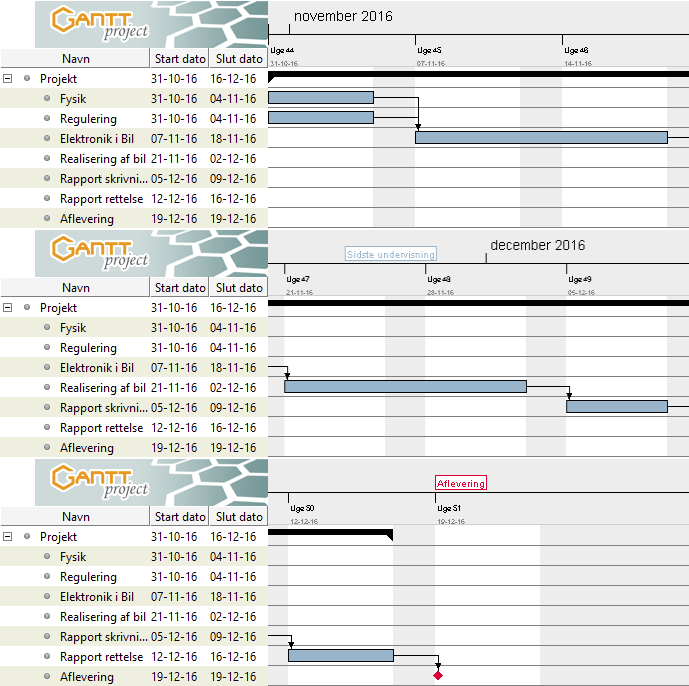
\includegraphics[width=0.2\textwidth]{gantt/gantt-cut.png}
	\caption{Tidsplanen over projektet}
	\label{fig:tidsplan}
\end{figure}

\husk{fraannk}{skal den ikke være lidt bredere? eller hva?}
\clearpage \newpage 
\section{Diagrammer af kredsløb i systemet} \label{bilag:diagrammer}

\husk{JJ}{Alle diagrammer fra Eagle her}

\newpage
\section{Oversigt af CD}\label{bilag:cd}
Oversigt af indholdet på den medfølgende cd. Beskrivelsen dækker kun det første mappeniveau og de underliggende filer kan fremstå i forskellig kvalitet og formater. Fodnoterne henviser til den nødvendige software, der skal bruges for at åbne filerne.

\begin{table}[h!]
\centering
\caption{Mappeoversigt af rapport CD}
\label{tab:ordliste}
\begin{threeparttable}
\begin{tabular}{l l}
\toprule
\multicolumn{1}{l}{Mappe}       &
\multicolumn{1}{l}{Beskrivelse}  \\ 
\midrule
Mappe					& Beskrivelse \\
\bottomrule
\end{tabular}
\begin{tablenotes}
\item[a] fodnote til mappe  \url{http://sdu.dk}
\end{tablenotes}
\end{threeparttable}
\end{table}




\end{document}